\chapter{Conclusions}
\label{cap:conclusions}
%   Savas

%   What did we do and whats the impact of the work we did for the company

This work analyses the strategic transformation of the Bank's IT Department toward a ``Shared Service Center'', operating model with the adoption of ITIL principles applyed to IT Service Management processes, and a KPI Based Management approach. \\
The international expansion of the organization, together with the integration of acquired financial institutions and collaboration with indipendent financial advisors, introduces significant challenges related to service standardization, operational efficiency, customer satisfaction, cost management and regulatory compliance. Consequently, the establishment of measurable performance mechanisms becomes essential to support strategic decision-making and ensure the long-term sustainability of IT services. \\
This document analyzed the Critical Successful Factors (\gls{csf}) individuated and provide respective KPI metrics to analyze and measures organizational processes thus to monitor and improve the value provided; as Figure ~\ref{fig:kpimetrics} illustrate, each CSF is composed by two related core topics and respectly the indicators deisgned.

%   Still WIP

\begin{figure}[h]
    \centering
    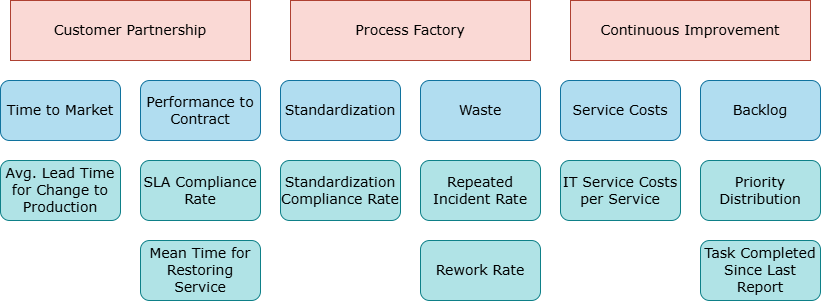
\includegraphics[width=0.8\textwidth]{images/metrics.png}
    \caption{KPI Metrics Relations Table}
    \label{fig:kpimetrics}
\end{figure}